\chapter{Introducción}
	
Este primer capítulo describe de forma general la información principal y relevante para poder comprender el funcionamiento del producto actual LUCA, así como los objetivos del proyecto a desarrollar junto con la explicación y motivación del mismo.
	
\section{Introducción}
	
	
En los últimos años, el volumen de datos que una empresa o entidad necesita o es capaz de gestionar o manipular ha aumentado de forma vertiginosa. Estos datos se almacenan en fuentes de diversos tipos, abarcando elementos tan dispares como bases de datos relacionales, hojas XML o repositorios FTP, a los cuales se accede mediante diferentes formas y lenguajes. Por tanto, un nuevo problema que debemos enfrentar, adicional al del volumen de datos a manipular, es que para acceder cierta información es necesario muchas veces establecer comunicaciones entre diferentes fuentes.

\vspace{5mm}
			
%%===================================================================%%
%% NOTE(Pablo): Meter aquí el ejemplo del resumen de nuevo, si se
%%              quiere más detallado
%%===================================================================%%

%% Init resumen

	 Como consecuencia de esta nueva situación, cuando un usuario	quiere obtener una información concreta cuyos datos residen en varios de estos
sistemas, necesita acceder a cada uno de estos sistemas, extraer de cada sistema la información que precisa, filtrarla y unificarla para finalmente	obtener los datos requeridos.

\vspace{5mm}

Por ejemplo, una tienda de electrodomésticos podría tener sistemas informáticos diferentes para el departamento de atención al cliente, para el departamento técnico de postventa y para el departamento de compras y adquisiciones.Por tanto, para conocer el estado actual de una reparación, podríamos necesitar:
\begin{itemize}
	\item  Acceder al primer sistema para obtener el identificador de la incidencia y en qué fase de su gestión se encuentra.
	\item  Comprobado que la incidencia está actualmente en reparación, recuperaríamos otro sistema el estado detallado de la reparación, comprobando que está a la espera de una pieza.
	\item Finalmente accederíamos al sistema de compra y adquisiciones para comprobar cuando está prevista la entrega de dicha pieza. Los sistemas de almacenamiento de la información pueden ser diversos, incluyendo desde un servicio web, una base de datos relacional, un repositorio de ficheros accesible vía FTP o una base de datos NoSQL.
\end{itemize}


\section{LUCA}

%% End resumen
			
Con el objetivo de facilitar este proceso de recuperación de información almacenada en sistemas y fuentes de datos hetereogéneas, dentro de la empresa CIC, se está desarrollando una aplicación denominada LUCA. Para facilitar este proceso de recuperación de información, LUCA proporciona un lenguaje común para todas las fuentes de datos a unificar, permitiendo al usuario abstraerse de los detalles de cada fuente.

\vspace{5mm}

%%===================================================================%%
%% NOTE(Pablo): Poner un ejemplo sencillo que muestre el
%%              funcionamiento de LUCA
%%===================================================================%%



%% Ejemplo Luca

A continuación se explica brevemente el funcionamiento de Luca con algunos ejemplo gráficos orientativos para ayudar a la comprensión del propio funcionamiento.

\vspace{5mm}

Para explicar el funcionamiento principal de dicho producto, se pretende describir el proceso de creación y ejecución de una consulta a un servicio REST.

\vspace{5mm}

En la vista inicial nos encontramos con una lista de consultas ya almacenadas, así como, una serie de filtros y opciones para la creación, ejecución y edición de consultas. Como se pretende explicar la creación y ejecución de una consulta, para avanzar en la vista se seleccionaría la creación de una nueva consulta.


\vspace{5mm}

A continuación, se muestra un ejemplo sobre un servicio REST, concretamente sobre el servicio REST de información de la flota de autobuses de Santander (TUS), donde tras introducir el identificador de una parada de autobús, se devolverá la información relativa a dicha parada, como es la localización.


	
	\begin{figure}[H]
		\centering
 		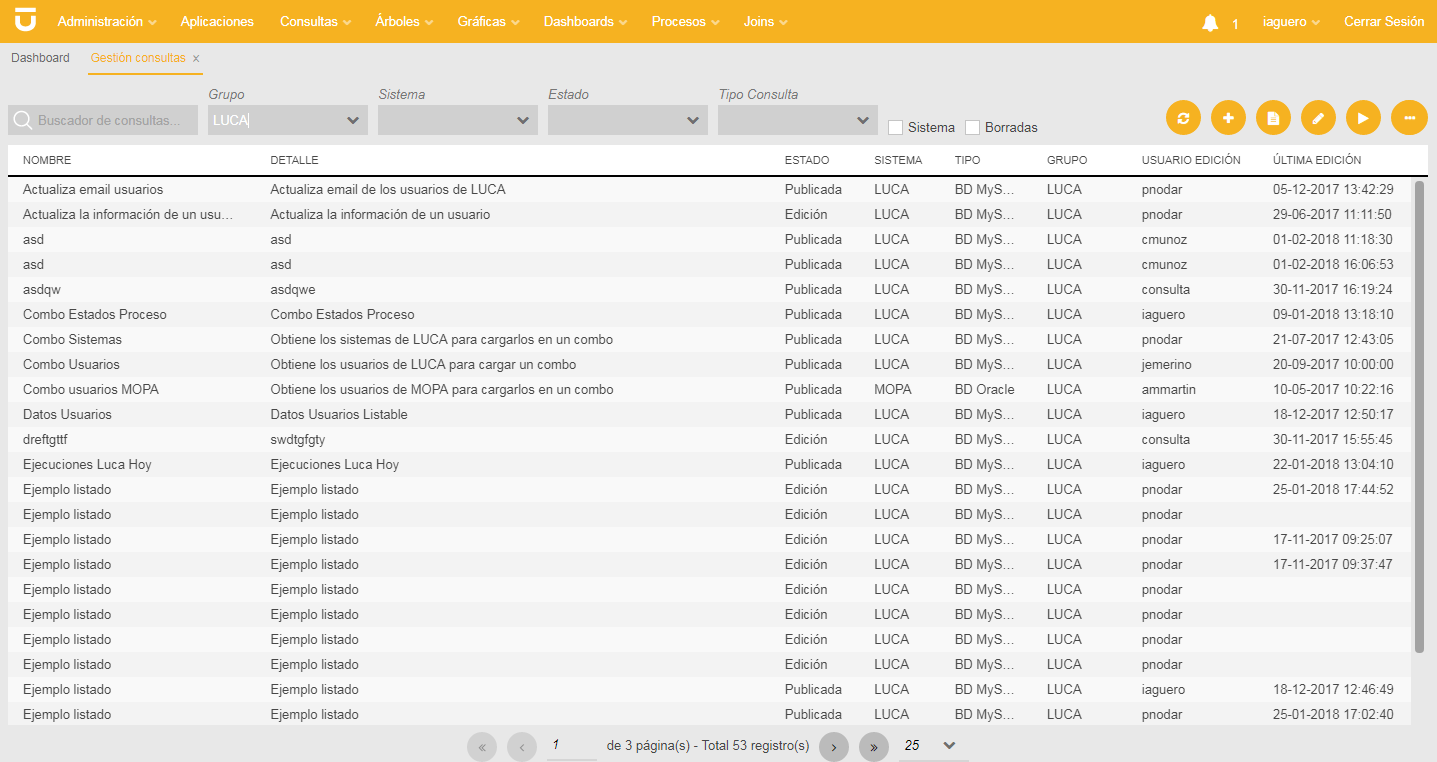
\includegraphics[scale=0.5]{capturasLuca/gestionConsultas.png}
		\caption{Vista de Gestión de Consultas}\label{fig:gestionConsulta}
	\end{figure}

Tras seleccionar la opción de creación de una nueva consulta, se muestra una vista en la que se permite agregar toda la información relativa a la consulta, como son las variables de entrada o de salida, o el tipo de salida que se desea recibir.

\vspace{5mm}

Una vez introducido el identificador de la parada, y seleccionado el botón de ejecución para llevar a cabo la ejecución de la consulta, se muestra el resultado de la consulta, el cuál puede ser visualizado de diferentes formas en función del recurso al que se llama.


	\begin{figure}[H]
		\centering
		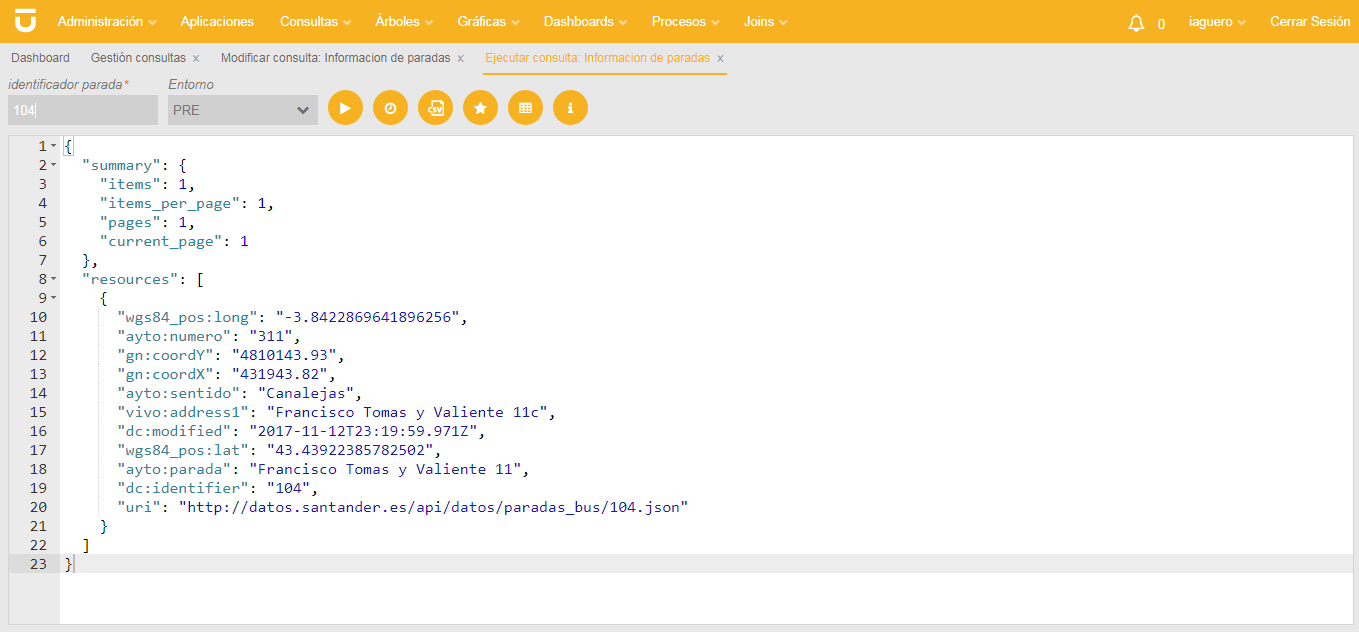
\includegraphics[scale=0.5]{capturasLuca/ejecucionConsulta.png}
		\caption{Vista de Ejecución de Consultas}\label{fig:ejecucionConsultas}
	\end{figure}


\vspace{5mm}


%% Fin ejemplo Luca

Actualmente LUCA proporciona mecanismos para permitir al usuario recuperar de manera uniforme información de diferentes fuentes de datos. No obstante, LUCA actualmente sólo es capaz recuperar información de una única fuente de datos a la vez. Por tanto, cuando es necesario combinar información procedente de distintas fuentes, el propio usuario es el que debe realizar dicho proceso de composición, ejecutando cada consulta a mano, y utilizando las salidas de cada una de ellas como las entradas de las siguientes.

\vspace{5mm}
			
%%===================================================================%%
%% NOTE(Pablo): Poner un ejemplo cómo es el proceso de composición
%%              a mano
%%===================================================================%%

Un ejemplo de dicho proceso de composición sería la necesidad de un dependiente de una tienda de electrodomésticos de obtener la edad de los usuarios que compraron lavadoras durante el mes pasado. Actualmente, los pasos o consecución de consultas que debería de realizar serían las siguientes:

\begin{itemize}
	\item  Primero necesitaría obtener el registro de compras del mes pasado del sistema.
	\item  Después, tras apuntarse dicho registro, tendría que, uno por uno, seleccionar los que se corresponden con lavadoras.
	\item Una vez que el usuario tiene las lavadoras compradas el mes pasado, éste tendría que recoger que usuarios han comprado las lavadoras.
	\item Por último, el usuario debería de buscar en el sistema cada usuario que ha realizado la compra, con el nombre obtenido previamente.
\end{itemize}

Se puede observar que el usuario tiene un engorroso desarrollo de acciones para poder obtener el resultado deseado.

\vspace{5mm}

%% Fin ejemplo composición

El objetivo de este proyecto es facilitar dicho proceso de composición al usuario mediante el desarrollo de un mecanismo gráfico para la especificación de estos procesos de composición de consultas.

\vspace{5mm}

%%===================================================================%%
%% NOTE(Pablo): Dar algunos detalles técnicos de cómo se pretente
%%              construir esto.
%%===================================================================%%
Para llevar a cabo esta tarea, se pretende realizar un sistema que permita visualmente utilizar las consultas ya almacenadas, para posteriormente relacionarlas entre sí mediante sus entradas y salidas y los tipos de las mismas. De esta forma, se podrá ejecutar automáticamente una cadena de consultas para obtener un resultado concreto, bajo un único concepto llamado Proceso.


\section{Ingeniería de Requisitos}

En esta sección se contará el proceso llevado a cabo para aprender o entender la estructuración y definición de requisitos de la actual LUCA, así como la propia descripción de los requisitos que serán necesarios para la implementación del proyecto a realizar.

\subsection{Proceso de integración en LUCA}

El primer paso llevado a cabo para la introducción en el producto de LUCA y entender así su funcionamiento, fue una reunión con el Jefe de Proyecto y con el Gerente para describir, analizar y explicar todos los aspectos de LUCA.

\subsection{Definición de Requisitos}

Una vez aclarados los términos del actual LUCA, se abordo el incremento que se quería llevar a cabo, del que parte este Trabajo de Fin de Grado. Se explicaron los términos de Proceso, variables de entradas y de salidas, consultas y demás.

\vspace{5mm}

Además de la explicación, se proporcionaron unos documentos técnicos tanto del componente gráfico del proceso como del incremento sobre LUCA. Estos documentos pueden encontrarse en el Anexo adjunto a la memoria.

\vspace{5mm}

Como ya se ha mencionado, en estos documentos se pueden encontrar los requisitos técnicos atribuidos al proyecto, pero, de forma resumida, se centran en tres pilares:

\begin{itemize}
	\item  Concatenación de las consultas entre si pertenecientes a un mismo proceso.
	\item  Visualización del progreso de ejecución del proceso.
	\item Aplicar criterios de navegación a partir de los resultados de salidas.
\end{itemize}

La especificación de estos requisitos se encuentra en los documentos técnicos citados anteriormente.


	 